\documentclass[10pt]{article}
\usepackage{fullpage}
\usepackage{amsmath}
\usepackage[amsthm, thmmarks]{ntheorem}
\usepackage{amssymb}
\usepackage{graphicx}
\usepackage{epstopdf}

\newtheorem{lemma}{Lemma}[section]
\newtheorem{theorem}[lemma]{Theorem}
\newtheorem{definition}[lemma]{Definition}
\newtheorem{proposition}[lemma]{Proposition}
\newtheorem{claim}[lemma]{Claim}

\newcommand{\dee}{\mathrm{d}}
\newcommand{\In}{\mathrm{in}}
\newcommand{\Out}{\mathrm{out}}
\newcommand{\pdf}{\mathrm{pdf}}
\newcommand{\Ei}{\mathrm{Ei}}

\title{Sampling Surface Points}
\author{Pramook Khungurn}

\begin{document}
	\maketitle
	
Given a point $x$ on a surface, we would like to sample
a point $y$ such that the the probability density that
$\| y - x \| = r$ is proportional to $f(r)$ for some fixed
function $f$.

\section{Motivation}

\begin{itemize}
	\item This sampling problem arises in the computation of outgoing radiance 
	from surface with subsurface scattering. 
	
	\item Let $x$ be a point on such a material. 
	The outgoing radiance at $x$ in direction $\omega$ is given by	
	\begin{align*}
		L_{\Out}(x, \omega) = 
		\int_A \int_{H^2} S(y,\omega' ,x,\omega) 
		L_{\In}(y, \omega') \cos \theta' \ \dee \omega' \dee y
	\end{align*}
	where
	\begin{itemize}
		\item $A$ is the surface where $x$ is on,
		\item $H^2$ is the hemisphere of direction around the surface normal at $x$,
		\item $S$ is the BFFRDF,
		\item $L_{\In}$	is the incoming radiance, and
		\item $\theta'$ is the angle between $\omega'$ and the surface normal.
	\end{itemize}

	\item The BSSRDF used is typically of the following form:
		$$ S(y,\omega_i,x,\omega_o) = T(\eta, \omega_i) 
		f(\| y-x \|) T(\eta,\omega_o)$$ 
	where
	\begin{itemize}
		\item $\eta$ is the index of refraction,
		\item $T(\eta,\omega)$ is the Fresnel transmittance, and
		\item $f$ is an arbitrary weight function.
	\end{itemize}
		
	\item We can evaluate the above integral by Monte Carlo 
	integration with importance sampling:
	\begin{align*}
		L_\Out(x, \omega) = \frac{1}{N} T(\eta, \omega) 
			\sum_{j=1}^N 
				\frac
				{
					f(r_j) L_i(y_j,\omega'_j) T(\eta, \omega') \cos \theta_j'
				}
				{ p(y_j, \omega'_j) }				
	\end{align*}
	where $p(y,\omega')$ is the probability density of sampling $y$ and 
	$\omega'$.

	\item To simplify the above sum, we want $p(y,\omega')$ to be 
	proportional to  $f(r) \cos \theta'$. That is, we want the 
	probability density of sampling $y$ be proportional to
	$f(r)$.
\end{itemize}

\section{The Sampling Algorithm}

\begin{itemize}
	\item Our sampling algorithm relies on the following fact.
	\begin{theorem} \label{intersection-sampling}
		Let $A$ be a flat surface that lies entirely in a
		sphere of radius $r$. 
		Pick two points $x_0$ and $x_1$ unifomly at random from 
		the surface of the sphere and draw a segment between them. 		
		Let $X$ be the number of points the segment intersects $A$. Then, 
		$$E[X] = \frac{A}{2\pi r^2}.$$
		In other words, the probability density that point $x$
		on the surface is on the segment as well is $1 / 2\pi r^2.$
	\end{theorem}	

	\item The above theorem suggest the following algorithm for uniformly
	sampling a point on a flat surface.	
		\begin{enumerate}
			\item Form a sphere that contains the surface.
			\item Pick two points uniformly at random from the surface of
				the sphere.
			\item Draw a segment between them.
			\item Report the intersection between the segment and the surface, 
				if there is one.
		\end{enumerate}
	
	\item Nevertheless, we would like to sample point $y$ around $x$ 
	such that the probability density of picking $y$ is proportional to 
	$f(r)$. We do so
	by a modified version of the previous algorithm.
		\begin{enumerate}
			\item Sample a number $s \in [0, \infty)$ according to
				another probability density function $g(s)$.
			\item Form a sphere of radius $s$ around $x$.
			\item Pick two points uniformly at random from the surface of
				the sphere.
			\item Draw a segment between them.
			\item Report the intersection between the segment and the surface, 
				if there is one.
		\end{enumerate}
		
	\item Let $y$ be a point on the surface at distance $r$ from $x$, and let $dA$ be an
		infinitesimal surface area containing $y$. We have that
		\begin{align*}
			\Pr(\mbox{pick $y$})
			&= f(r)\ \dee A \\
			&= \int_{0}^\infty \Pr(\mbox{pick $s$}) \Pr(\mbox{pick $y$}\ |\ \mbox{pick $s$})\ \dee s \\
			&= \int_{0}^\infty g(s) \Pr(\mbox{pick $y$}\ |\ \mbox{pick $s$})\ \dee s\\
			&= \int_{0}^r g(s) \Pr(\mbox{pick $y$}\ |\ \mbox{pick $s$})\ \dee s
				+ \int_{r}^\infty g(s) \Pr(\mbox{pick $y$}\ |\ \mbox{pick $s$})\ \dee s
		\end{align*}
		When $s < r$, the probability of picking $y$ is $0$. Otherwise, the 
		probability is $\dee A / (2\pi s^2).$ Hence,
		\begin{align*}
			f(r)\ \dee A &= \int_{r}^\infty g(s) \frac{\dee A}{2\pi s^2}\ \dee s\\
			f(r) &= \int_{r}^\infty \frac{g(s)}{2\pi s^2}\ \dee s\\
			-f(r) &= \int_\infty^{r} \frac{g(s)}{2\pi s^2}\ \dee s
		\end{align*}
		Differentiating both sides with $r$, we have
		\begin{align*}
			-f'(r) &= \frac{g(r)}{2\pi r^2}\\
			g(r) &= -2\pi r^2 f'(r).
		\end{align*}
	
	\item In order for $g(r)$ to be a probability density, $f'(r)$ must be non-positive,
		which means that $f$ must be non-increasing. Moreover, $\int_0^\infty g(r)\ \dee r$
		must be 1. Now,
		\begin{align*}
			\int_0^\infty g(r)\ \dee r &= \int_0^\infty -2\pi r^2 f'(r)\ \dee r\\
			1 &= - 2\pi \bigg[ r^2 f(r) \bigg]_0^\infty + 4\pi \int_0^\infty r f(r)\ \dee r.
		\end{align*}
		If we require that $\lim_{r \rightarrow \infty} r^2 f(r) = 0,$ 
		we have that
		\begin{align*}
			1 = 4\pi \int_0^\infty r f(r)\ \dee r = 2 \int_0^{2 \pi} \int_0^\infty f(r) r\ \dee r \dee \phi = 2\int_A f(r)\ \dee A.
		\end{align*}
		In other words, $$\int_A f(r)\ \dee A = \frac{1}{2},$$
		or the weight function must integrate to one half on the whole plane.
		
	\item \begin{theorem}
		Let $f: \mathbb{R}^2 \rightarrow \mathbb{R}$ be such that $f(y)$ 
		depends only on the distance between $y$ and the origin. 
		(That is, we can write $f(y) = f(r)$ where $r$ is the distance.)
		Moreover, let $f$ satisfies the following properties:
		\begin{itemize}
			\item $f$ is not increasing in $r$,
			\item $\lim_{r \rightarrow \infty} r^2 f(r) = 0$, and
			\item $\int_A f(r)\ \dee y = 1/2$.
		\end{itemize}
		If we sample the radius $s$ of the sphere according to probability
		density funcion $$g(r) = -2\pi r^2 f'(r),$$
		then the probability density point $y$ at distance $r$ from $x$ gets
		picked is $f(r).$
	\end{theorem}
	
	\item When sampling the radius $s$, we need to evaluate the cumulative
	distribution function of $g$. This is given by
	$$\int_0^r g(r)\ \dee r = - 2\pi r^2 f(r) + 4\pi \int_0^r sf(s)\ \dee s.$$
\end{itemize}

\section{Sampling Distribution for Some Weight Function}

\subsection{Uniform Weight}
\begin{itemize}
	\item If we want every point inside a circle of radius $R$
		centered at $x$ to have equal weight, we choose
		\begin{align*}
			f(r) = \begin{cases}
				1/(2\pi R^2), & 0 \leq r \leq R \\
				0, & r > R
			\end{cases}.
		\end{align*}
	\item Hence,
		\begin{align*}
			g(r) = 2\pi r^2 f(r) = \begin{cases}
				0, & 0 \leq r < R \\
				\delta(r - R)/(2\pi R^2), & r = R \\
				0, & r > R
			\end{cases}.
		\end{align*}
		This $g$ suggests that we set $s = R$, which makes perfect sense.
\end{itemize}

\subsection{Polynomial Weight 1}
\begin{itemize}
	\item In this section, we want $f$ be proportional to 
		\begin{align*}
			f^*(r) = \begin{cases}
				(1 - r/R)^d, & 0 \leq r \leq R \\
				0, & r > R
			\end{cases}
		\end{align*}
		We want to find a constant $c$ such that 
		$\int_A c(1 - r/R)^d\ \dee A = \frac{1}{2}.$ 
		We have that
		\begin{align*}
			\int_A (1 - r/R)^d\ \dee A 
			&= \int_0^\infty \int_0^{2\pi} r(1 - r/R)^d\ \dee \phi \dee r\\
			&= 2\pi \int_0^{R} r(1- r/R)^d \ \dee r\\
			&= 2\pi \bigg( \bigg[ - \frac{Rr(1-r/R)^{d+1}}{d+1}\bigg]_0^R 
				- \int_0^R \frac{-R(1-r/R)^{d+1}}{d+1}\ \dee r \bigg)\\
			&= -2\pi \bigg[ \frac{R^2(1-r/R)^{d+2}}{(d+1)(d+2)} \bigg]_0^R\\
			&= \frac{2\pi R^2}{(d+1)(d+2)}.
		\end{align*}
		So, $c = (d+1)(d+2) / (4\pi R^2)$ and 
		$$f(r) = \frac{(d+1)(d+2)(1 - r/R)^d}{4 \pi R^2}\mbox{, $0 \leq r \leq R$}$$
		\begin{figure}[h]
			\centering
			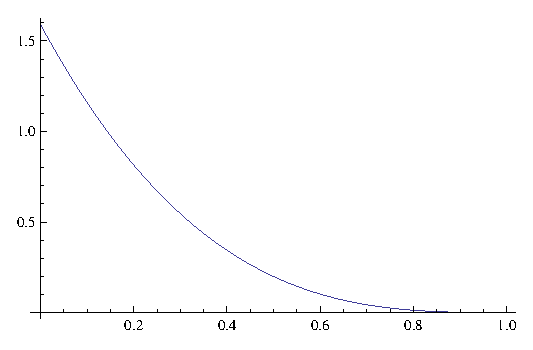
\includegraphics{cubic.eps}
			\caption{The weight function propotional to $(1-r/R)^3$ with $R = 1$.}
		\end{figure}
	\item The probability distribution $g$ is then
		\begin{align*}
			g(r) 
			&= -2\pi r^2 f'(r)\\
			&= -2\pi r^2
				\bigg[ \frac{(d+1)(d+2)(1 - r/R)^d}{4\pi R^2} \bigg]'\\
			&= \frac{d(d+1)(d+2)}{2R^3} r^2 (1-r/R)^{d-1}\mbox{, $0 \leq r \leq R$}.
		\end{align*}
		The cumulative distribution function is
		\begin{align*}
			\int_0^r g(r)\ \dee r
			&= \frac{d(d+1)(d+2)}{2R^3} \int_0^r s^2(1-s/R)^{d-1}\ \dee s\\
			&= \frac{d(d+1)(d+2)}{2R^3} \bigg[ -\frac{R (1-s/R)^d (2R^2 + 2Rds + d(d+1)s^2) }{d(d+1)(d+2)} \bigg]_0^r\\
			&= \frac{1}{2R^2} 
				\bigg[ -(1-s/R)^d (2R^2 + 2Rds + d(d+1)s^2) \bigg]_0^r\\
			&= 1 - \frac{(1-r/R)^d(2R^2 - 2Rdr + d(d+1)r^2)}{2R^2}\\
			&= 1 - (1-r/R)^d \bigg( 1 - \frac{d}{R}r 
				+ \frac{d(d+1)}{2R^2}r^2 \bigg)\mbox{, $0 \leq r \leq R$}.
		\end{align*}
\end{itemize}

\subsection{Polynomial Weight 2}
\begin{itemize}
	\item  In this section, we want $f$ be proportional to 
		\begin{align*}
			f^*(r) = \begin{cases}
				1 - (r/R)^d, & 0 \leq r \leq R \\
				0, & r > R
			\end{cases}
		\end{align*}
		We want to find a constant $c$ such that 
		$\int_A c(1 - (r/R)^d)\ \dee A = \frac{1}{2}.$ 
		We have that
		\begin{align*}
			\int_A (1 - (r/R)^d)\ \dee A 
			&= \int_0^\infty \int_0^{2\pi} r(1 - (r/R))^d\ \dee \phi \dee r\\
			&= 2\pi \int_0^{R} r(1- (r/R)^d) \ \dee r = 2\pi \bigg( \int_0^{R} r\ \dee r - \int_0^R r^{d+1}/R^d\ \dee r \bigg)\\
			&= 2\pi \bigg( \bigg[ \frac{r^2}{2} \bigg]_0^R - \bigg[ \frac{r^{d+2}}{(d+2)R^d} \bigg]_0^R \bigg)\\
			&= 2\pi \bigg( \frac{R^2}{2} - \frac{R^2}{d+2} \bigg)\\
			&= \frac{\pi d R^2}{d+2}.
		\end{align*}
		So, $c = (d+2) / (2\pi d R^2)$ and 
		$$f(r) = \frac{d+2}{2 \pi d R^2}\bigg(1 - \frac{r^d}{R^d}\bigg)\mbox{, $0 \leq r \leq R$}$$
		\begin{figure}[h]
			\centering
			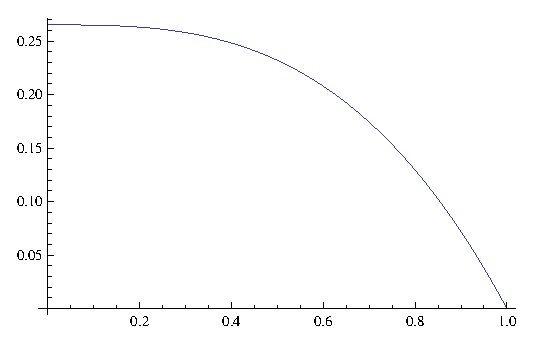
\includegraphics{one-minus-cubic.eps}
			\caption{The weight function proportional to $1 - (r/R)^3$ with $R = 1$.}
		\end{figure}
	\item The probability density function is then
		\begin{align*}
			g(r) 
			&= -2\pi r^2 f'(r) = - 2\pi r^2 \times \frac{d+2}{2\pi d R^2} \times (-d) \frac{r^{d-1}}{R^d} = \frac{d+2}{R^{d+2}}r^{d+1}.
		\end{align*}
	
	\item The cdf is
		\begin{align*}
			\int_0^r g(s)\ \dee s = \frac{d+2}{R^{d+2}} \int_0^r r^{d+1} \ \dee r =  \frac{d+2}{R^{d+2}} \bigg[ \frac{s^{d+2}}{d+2} \bigg]_0^r
			= \frac{r^{d+2}}{R^{d+2}}.
		\end{align*}
\end{itemize}

\subsection{Polynomial Weight 3}
\begin{itemize}
	\item In this section, we want $f$ to be proportional to
		\begin{align*}
			f^*(r) = \begin{cases}
				(1 - r^2/R^2)^2, & 0 \leq r \leq R, \\
				0, & r > 1
			\end{cases}
		\end{align*}
	\item Integrating $f^*(r)$ over the plane, we have
		\begin{align*}
			\int_0^{2\pi} \int_0^\infty r f^*(r)\ \dee r \dee \theta
			&= 2\pi \int_0^R r (1-r^2/R^2)^2\ \dee r
			= 2\pi \int_0^R \bigg( r - \frac{2r^3}{R^2} + \frac{r^5}{R^4} \bigg)\ \dee r\\
			&= 2\pi \bigg( \bigg[ \frac{r^2}{2} \bigg]_0^R 
				- \bigg[ \frac{r^4}{2R^2} \bigg]_0^R 
				+ \bigg[ \frac{r^6}{6R^4} \bigg]_0^R \bigg)\\
			&= 2\pi \bigg( \frac{R^2}{2} - \frac{R^2}{2} + \frac{R^2}{6} \bigg)
			= \frac{\pi R^2}{3}.			
		\end{align*}
		Hence, $$f(r) = \frac{3(1 - r^2/R^2)^2}{2\pi R^2}.$$

		\begin{figure}[h]
			\centering
			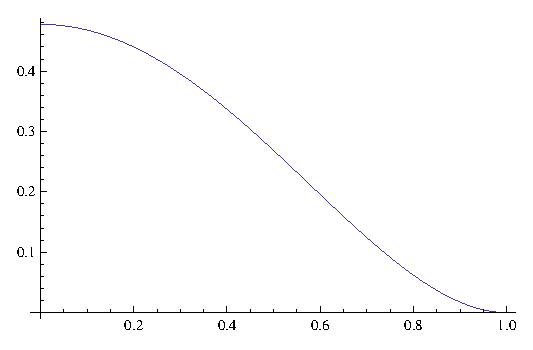
\includegraphics{one-minus-square-squared.eps}
			\caption{The weight function proportional to $(1 - (r/R)^2)^2$ with $R = 1$.}
		\end{figure}
	
	\item We have that 
		\begin{align*}
			g(r) 
			&= -2\pi r^2 f'(r) = -\frac{3}{R^2} r^2 \{ (1 - r^2/R^2)^2 \}'
			= -\frac{3}{R^2} r^2 \bigg\{ 1 - \frac{2r^2}{R^2} + \frac{r^4}{R^4} \bigg\}'
			= -\frac{3}{R^2} r^2 \bigg(  -\frac{4r}{R^2} + \frac{4r^3}{R^4} \bigg)\\
			&= 12 \bigg( \frac{r^3}{R^4} - \frac{r^5}{R^6} \bigg)
		\end{align*}
		
	\item The cdf is then:
		\begin{align*}
			\int_0^r g(s)\ \dee s 
			&= \frac{12}{R^4} \int_0^r s^3\ \dee s - 
			\frac{12}{R^4} \int_0^r s^5\ \dee s\\
			&= \frac{12}{R^6} \frac{r^4}{4} 
				- \frac{12}{R^6}\frac{r^6}{6}
			= \frac{3r^4}{R^4} - \frac{2r^6}{R^6}.
		\end{align*}
		One nice thing about this cdf is that it is a cubic polynomial
		in $r^2/R^2$, which means we can solve $\int_0^r g(s)\ \dee s = \xi$
		for any given $\xi$ exactly.
\end{itemize}

\subsection{Exponential Weight}
\begin{itemize}
	\item In this section, we want $f$ be proportional to 
		\begin{align*}
			f^*(r) = e^{-\sigma r}.
		\end{align*}
		for some positive constant $\sigma$.
		We want to find a constant $c$ such that 
		$\int_A ce^{-\sigma r}\ \dee A = \frac{1}{2}.$ 
		We have that
		\begin{align*}
			\int_A e^{-\alpha r}\ \dee A 
			&= \int_0^\infty \int_0^{2\pi} e^{-\sigma r}\ \dee \phi \dee r\\
			&= 2\pi \int_0^{\infty} e^{-\sigma r} \ \dee r\\
			&= 2\pi \bigg[ - 
				\frac{e^{-\sigma r}(\sigma r  + 1)}{\sigma^2} \bigg]_0^\infty\\
			&= 2\pi /\sigma^2.
		\end{align*}
		So, $c = \sigma^2 / (4\pi)$ and 
		$$f(r) = \frac{\sigma^2 e^{-\sigma r}}{4\pi} $$

		\begin{figure}[h]
			\centering
			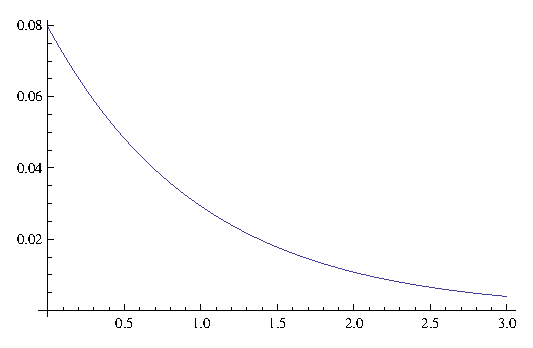
\includegraphics{exponential.eps}
			\caption{The weight function proportional to $e^{-\sigma r}$ with $\sigma = 1$.}
		\end{figure}		
	
	\item The probability distribution $g$ is then
		\begin{align*}
			g(r) 
			&= -2\pi r^2 f'(r)\\
			&= \frac{\sigma^3 r^2}{2} e^{-\sigma r}.
		\end{align*}
		The cumulative distribution function is
		\begin{align*}
			\int_0^r g(r)\ \dee r
			&= \frac{\sigma^3}{2} \int_0^r s^2 e^{-\sigma s}\ \dee s\\
			&= \frac{\sigma^3}{2} 
				\bigg[ - \frac{1}{\sigma^3} e^{-\sigma s} 
				(\sigma^2 s^2 + 2\sigma s + 2)\bigg]_0^r\\
			&= \frac{1}{2} 
				\bigg[- e^{-\sigma s} 
				(\sigma^2 s^2 + 2\sigma s + 2) \bigg]_0^r\\
			&= 1 - \frac{1}{2} e^{-\sigma r} 
				(\sigma^2 r^2 + 2\sigma r + 2).
		\end{align*}
\end{itemize}
		
\subsection{Jensen's Dipole Weight}
\begin{itemize}
	\item A popular weight to use is the dipole diffuse scattering weight.
		The dipole weight function has four parameters:
		\begin{itemize}
			\item the coefficient of absorption $\sigma_a$,
			\item the coefficient of scattering $\sigma_s$,
			\item the mean cosine $g$, and
			\item the index of refraction $\eta$.			
		\end{itemize}
		From these parameters, we define the following quantities:
		\begin{itemize}
			\item $\sigma_s' = \sigma_s (1 - g)$,
			\item $\sigma_t' = \sigma_s' + \sigma_a$,
			\item $D = \frac{1}{3 \sigma_t'}$,
			\item $F_{dr} = \frac{-1.44}{\eta^2} + \frac{0.71}{\eta} + 0.668 + 0.0636\eta$,
			\item $A = \frac{1+F_{dr}}{1-F_{dr}}$,
			\item $\sigma = \sqrt{3 \sigma_a \sigma_t' }$,
			\item $z_r = 1 / \sigma_t'$,
			\item $z_v = z_r + 4AD$, and
			\item $\alpha' = \sigma_s' / \sigma_t'$.
		\end{itemize}
		Then, the dipole weight is given by:
		\begin{align*}
			f^*(r) = \frac{\alpha'}{4\pi} 
			\bigg[ z_r( \sigma (r^2 + z_r^2)^{1/2} + 1) 
			\frac{e^{-\sigma (r^2 + z^2_r)^{1/2}}}{(r^2 + z^2_r)^{3/2}} + 
			z_v( \sigma (r^2 + z_v^2)^{1/2} + 1) 
			\frac{e^{-\sigma (r^2 + z^2_v)^{1/2}}}{(r^2 + z^2_v)^{3/2}} \bigg]
		\end{align*}
		
		\begin{figure}[h]
			\centering
			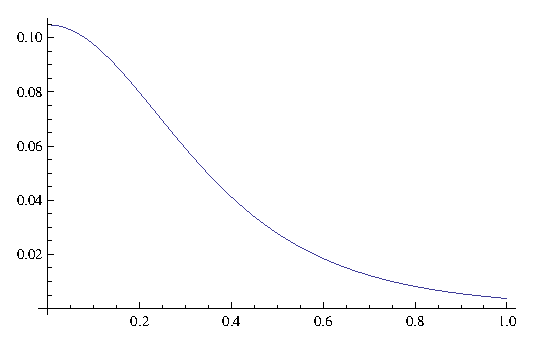
\includegraphics{dipole.eps}
			\caption{The (unnormalized) dipole weight function with $\sigma_a = \sigma_s = 1$, $g = 0$, and $\eta = 1.2$.}
		\end{figure}
		
	\item Let 
		\begin{align*}
			h(r,z) = (\sigma (r^2 + z^2)^{1/2} + 1) 
			\frac{
				e^{-\sigma (r^2+z^2)^{1/2}}
			}
			{(r^2 + z^2)^{3/2}}.		
		\end{align*}
		We have that 
		\begin{align*}
			\int r h(r,z)\ \dee r = -\frac{
				e^{-\sigma (r^2+z^2)^{1/2}}}
				{(r^2 + z^2)^{1/2}} + C
		\end{align*}
	
	\item Rewriting $f^*(r)$, we have
		$$f^*(r) = \frac{\alpha'}{4\pi}[ z_r h(r, z_r) + z_v h(r, z_v) ].$$			Let us integrate $f^*(r)$ over the plane.
		\begin{align*}
			\int_0^\infty \int_0^{2\pi} rf^*(r)\ \dee\phi \dee r
			&= 2\pi \int_0^\infty rf^*(r)\ \dee r\\
			&= \frac{\alpha'}{2} 
				\bigg( 
				z_r \int_0^\infty r h(r, z_r) \ \dee r +
				z_v \int_0^\infty r h(r, z_v) \ \dee v
				\bigg)\\
			&= \frac{\alpha'}{2} \bigg( 
				z_r \bigg[ -\frac{e^{-\sigma (r^2+z_r^2)^{1/2}}}
				{(r^2 + z_r^2)^{1/2}} \bigg]_0^\infty 
				+ z_v \bigg[ -\frac{e^{-\sigma (r^2+z_v^2)^{1/2}}}
				{(r^2 + z_v^2)^{1/2}} \bigg]_0^\infty \bigg)\\
			&= \frac{\alpha'}{2}(e^{-\sigma z_r} + e^{-\sigma z_v}).			
		\end{align*}
		
	\item So, the weight function $f$ is 
		$$f(r) 
		= \frac{1}{2} \times \frac{2}{\alpha'(e^{-\sigma z_r} + e^{-\sigma z_v})} \times f^*(r)
		= \frac{z_r h(r,z_r) + z_v h(r,z_v)}{4\pi(e^{-\sigma z_r} + e^{-\sigma z_v})}.$$
	
	\item Since the calculation of $g$ is a pain in the neck, we compute
		the cdf of $g$ instead. Recall from last section that
		\begin{align*}			
		\int_0^r g(r)\ \dee r 
		&= - 2\pi r^2 f(r) + 4\pi \int_0^r sf(s)\ \dee s.		
		\end{align*}
		Let us work on the above expression term by term.
		For the first time, we have
		\begin{align*}
			-2\pi r^2 f(r) 
			&= -2\pi r^2 \bigg( \frac{z_r h(r,z_r) + z_v h(r,z_v)}{4\pi(e^{-\sigma z_r} + e^{-\sigma z_v})} \bigg)
			= -r^2 \bigg( \frac{z_r h(r,z_r) + z_v h(r,z_v)}{2(e^{-\sigma z_r} + e^{-\sigma z_v})} \bigg).
		\end{align*}
		For the second term, we have
		\begin{align*}
			4\pi \int_0^r sf(s)\ \dee s
			&= 4\pi \int_0^r s \frac{z_r h(s,z_r) + z_v h(s,z_v)}{4\pi(e^{-\sigma z_r} + e^{-\sigma z_v})}\ \dee s\\
			&= \frac{1}{e^{-\sigma z_r} + e^{-\sigma z_v}}
			\int_0^r z_r s h(s,z_r) + z_v s h(s,z_v)\ \dee s\\
			&= \frac{1}{e^{-\sigma z_r} + e^{-\sigma z_v}}
			\bigg[ -z_r \frac{
				e^{-\sigma (s^2+z_r^2)^{1/2}}}
				{(s^2 + z_r^2)^{1/2}} 
				- z_v \frac{
				e^{-\sigma (s^2+z_v^2)^{1/2}}}
				{(s^2 + z_v^2)^{1/2}} \bigg]_0^r\\
			&= 1  - \frac{1}{e^{-\sigma z_r} + e^{-\sigma z_v}}
			 \bigg( z_r \frac{
				e^{-\sigma (r^2+z_r^2)^{1/2}}}
				{(r^2 + z_r^2)^{1/2}} 
				+ z_v \frac{
				e^{-\sigma (r^2+z_v^2)^{1/2}}}
				{(r^2 + z_v^2)^{1/2}} \bigg).
		\end{align*}
		Then,
		\begin{align*}
			\int_0^r g(r)\ \dee r 
			&= 1 - \frac{1}{e^{-\sigma z_r} + e^{-\sigma z_v}}
			 \bigg( z_r \frac{
				e^{-\sigma (r^2+z_r^2)^{1/2}}}
				{(r^2 + z_r^2)^{1/2}} 
				+ z_v \frac{
				e^{-\sigma (r^2+z_v^2)^{1/2}}}
				{(r^2 + z_v^2)^{1/2}} \bigg)
				 -r^2 \bigg( \frac{z_r h(r,z_r) + z_v h(r,z_v)}{2(e^{-\sigma z_r} + e^{-\sigma z_v})} \bigg).
		\end{align*}
\end{itemize}

\pagebreak
\section{Images}
\begin{figure}[h]
	\centering
	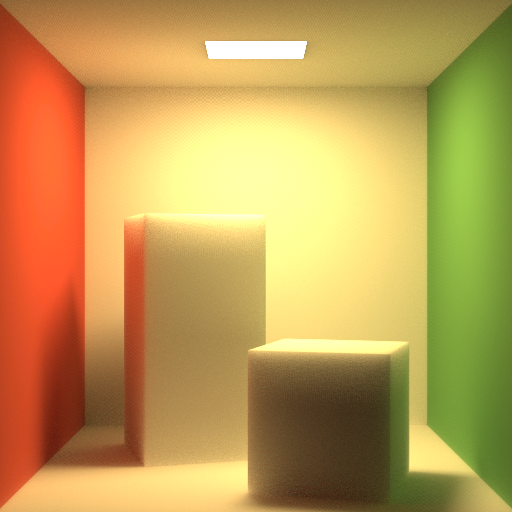
\includegraphics[height=160mm]{cubic.png}
	\caption{$f(r) \propto (1-r/80)^3$}
\end{figure}

\begin{figure}[h]
	\centering
	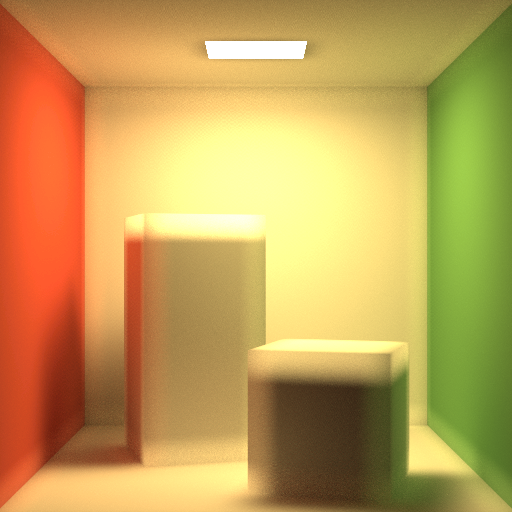
\includegraphics[height=160mm]{one-minus-cubic.png}
	\caption{$f(r) \propto 1-r^3/40^3$}
\end{figure}

\begin{figure}[h]
	\centering
	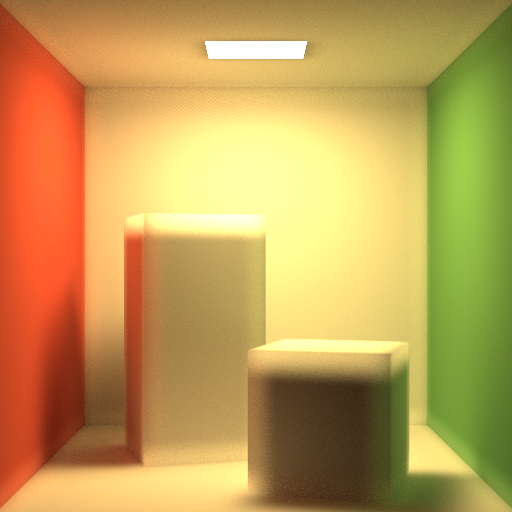
\includegraphics[height=160mm]{one-minus-square-squared.png}
	\caption{$f(r) \propto (1-r^2/40^2)^2$}
\end{figure}

\begin{figure}[h]
	\centering
	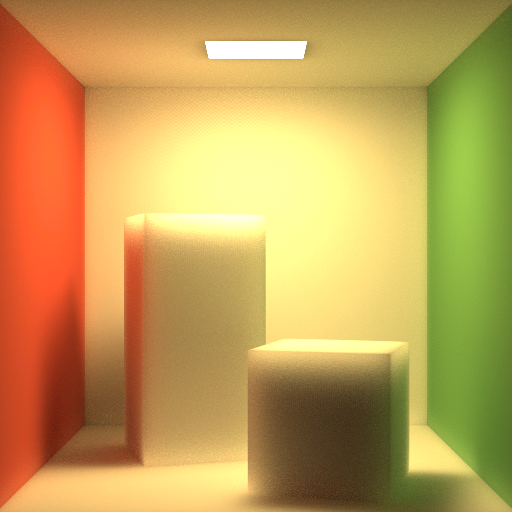
\includegraphics[height=160mm]{exponential.png}
	\caption{$f(r) \propto e^{-0.1r}$}
\end{figure}

\begin{figure}[h]
	\centering
	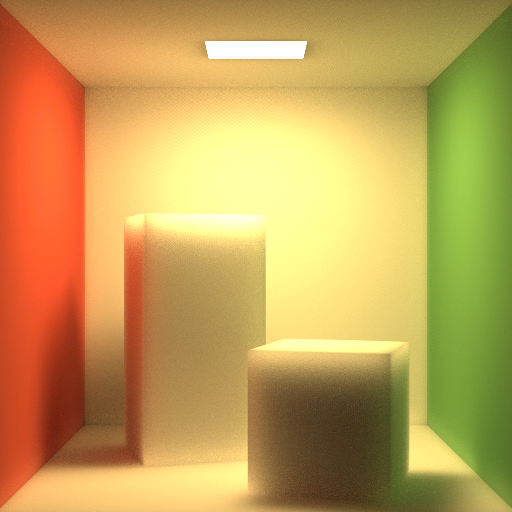
\includegraphics[height=160mm]{dipole.png}
	\caption{Dipole weight function with $\sigma_s = \sigma_a = 0.025$, $g = 0$, $\eta = 1.2$. I'm shocked it looks almost the same as the exponential weight function.}
\end{figure}

\end{document}